% use the answers clause to get answers to print; otherwise leave it out.
%\documentclass[11pt,answers]{exam}
\documentclass[11pt]{exam}
\RequirePackage{amssymb, amsfonts, amsmath, latexsym, verbatim, xspace, setspace}
\usepackage{graphicx}

% By default LaTeX uses large margins.  This doesn't work well on exams; problems
% end up in the "middle" of the page, reducing the amount of space for students
% to work on them.
\usepackage[margin=1in]{geometry}
\usepackage{enumerate}
\usepackage[hidelinks]{hyperref}

% Here's where you edit the Class, Exam, Date, etc.
\newcommand{\class}{NPRE 555}
\newcommand{\term}{Fall 2020}
\newcommand{\assignment}{CP 3}
\newcommand{\duedate}{2020.12.14}
%\newcommand{\timelimit}{50 Minutes}

\newcommand{\nth}{n\ensuremath{^{\text{th}}} }
\newcommand{\ve}[1]{\ensuremath{\mathbf{#1}}}
\newcommand{\Macro}{\ensuremath{\Sigma}}
\newcommand{\vOmega}{\ensuremath{\hat{\Omega}}}

% For an exam, single spacing is most appropriate
\singlespacing
% \onehalfspacing
% \doublespacing

% For an exam, we generally want to turn off paragraph indentation
\parindent 0ex

%\unframedsolutions

\begin{document} 

% These commands set up the running header on the top of the exam pages
\pagestyle{head}
\firstpageheader{}{}{}
\runningheader{\class}{\assignment\ - Page \thepage\ of \numpages}{Due \duedate}
\runningheadrule

\class \hfill \term \\
\assignment \hfill Due \duedate\\
\rule[1ex]{\textwidth}{.1pt}
%\hrulefill

%%%%%%%%%%%%%%%%%%%%%%%%%%%%%%%%%%%%%%%%%%%%%%%%%%%%%%%%%%%%%%%%%%%%%%%%%%%%%%%%%%%%%
%%%%%%%%%%%%%%%%%%%%%%%%%%%%%%%%%%%%%%%%%%%%%%%%%%%%%%%%%%%%%%%%%%%%%%%%%%%%%%%%%%%%%
\begin{itemize}
        \item Show your work. 
        \item This work must be submitted online via github classroom at 
                \url{https://classroom.github.com/a/LvxO8rBo}. 
        \item All code must be version controlled with git in addition to the 
                report \texttt{.pdf} and presentation \texttt{.pdf}.
        \item This project should be individual work.
\end{itemize}
\rule[1ex]{\textwidth}{.1pt}


% ---------------------------------------------
\begin{questions}
        % ---------------------------------------------

        \question[30] Select\footnote{Please select something other than Monte Carlo, $P_N$, or $S_N$. In order to choose one of these you must add advanced features (e.g. coarse mesh rebalancing) and address a challenging problem (e.g. 3-D cylinder).} and implement a neutron transport method.  
        Report on your results with sufficient clarity to reproduce your work. This should include a clear README describing how your instructor can replicate your work. A report document (in  \texttt{.pdf} format) should include a 4 (or more) page description of your method and results. Scanned handwritten documents will not be accepted. The report must be generated by a typesetting program (Markdown or LaTeX generated documents are preferred but Word, Open Office, Google Docs are allowed).
        \begin{parts} 
                \part Consider finding a straightforward paper concerning a 
                simple geometry and replicating its results.
                \part Include references 
                to primary sources (journal articles).
                \part Clearly explain in your report what approximations 
                your method makes (energy, angle, space). 
                \part Summarize the current use of this method.
                \part Describe the strengths and weaknesses of the method as 
                 well as the kinds of problems for which it is and is not 
                 appropriate.
        \end{parts}

        % ---------------------------------------------
        \question[20] Solve for the flux in a basic problem see Section 
        \ref{sec:basic}.

        % ---------------------------------------------
        \question[30] Go further. Select two challenge problems from Section 
\ref{sec:challenge}.

        % ---------------------------------------------
        \question[20] Prepare a 10 minute presentation and present to the class 
        at 8am December 14th. Include a \texttt{.pdf} of the presentation in the repository.

\end{questions}

\pagebreak

\section{Basic Problems}\label{sec:basic}
   \subsection{Slab Scalar Flux} 
   Solve for the scalar flux as a function of space in an infinite slab with 
   two regions in Figure \ref{fig:slab}.  There are vacuum boundary conditions 
   on both sides of the slab.  Scattering is isotropic in the lab system.  
        In region 1:
        \begin{itemize}
                \item Width is $2cm$.
                \item $\Sigma_t = \frac{1}{cm}$.
                \item $\Sigma_a = \frac{0.5}{cm}$.
                \item There is a uniformly distributed isotropic unit source $\left(1\left[\frac{n}{cm}\right]\right)$.
        \end{itemize}


        In region 2:
        \begin{itemize}
                \item Width is $4cm$.
                \item $\Sigma_t = \frac{1.5}{cm}$.
                \item $\Sigma_a = \frac{1.2}{cm}$.
                \item There is no source.
        \end{itemize}

        \begin{figure}[htb!]
                \begin{center}
                        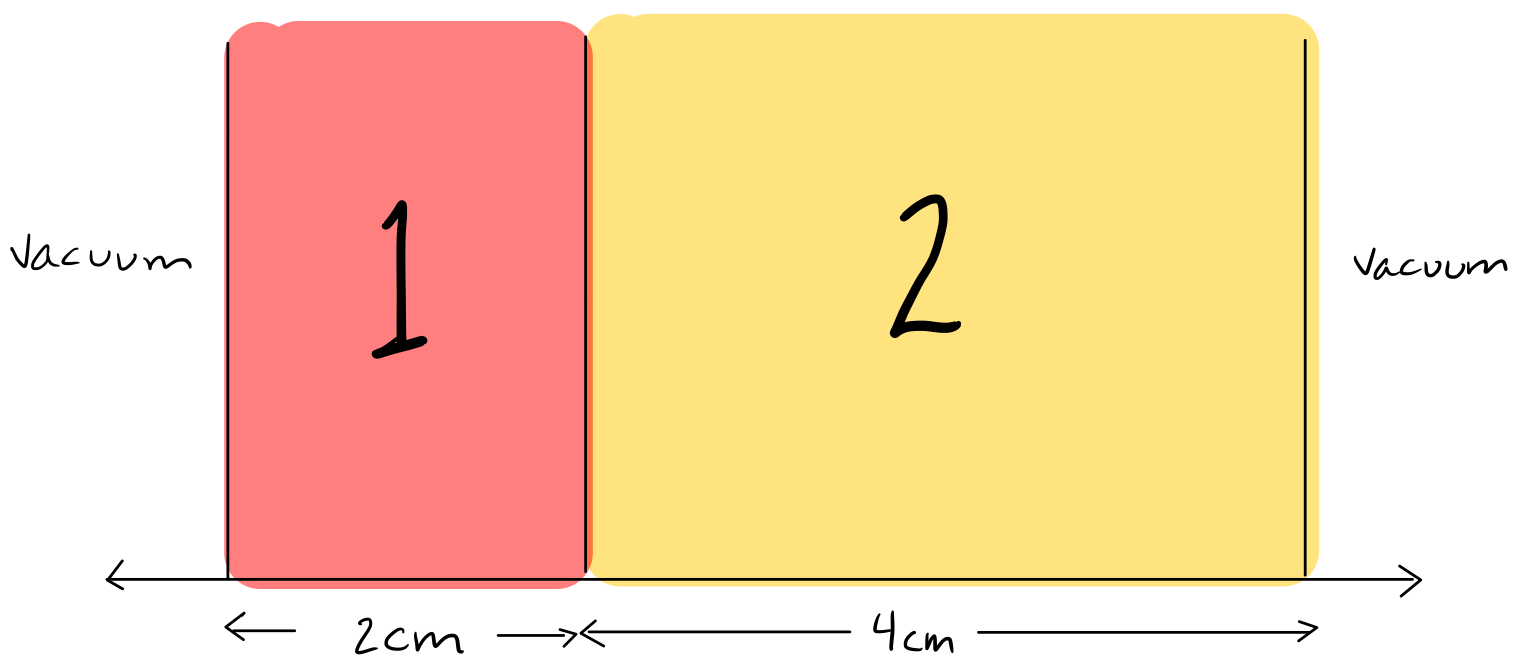
\includegraphics[width=0.5\textwidth]{slab-prob.png}
                \end{center}
                \caption{Infinite slab with two regions.}
                \label{fig:slab}
        \end{figure}

        \subsection{Slab Angular Flux}
        Consider a slab
        \begin{itemize}
                \item $\Sigma_t = \frac{1}{cm}$.
                \item $\Sigma_a = \frac{0.5}{cm}$.
                \item There is a uniformly distributed isotropic unit source $\left(S_0\left[\frac{n}{cm}\right]\right)$.
                \item The slab has length L
                \item The slab has vacuum boundaries.
        \end{itemize}

        Find the rightward angular flux $\psi_+$, leftward angular
        flux $\psi_-$, the scalar flux $\phi(x)$

        Plot the angular flux from $0\le x \le L$ for values of $\mu$ corresponding to
        $\theta = \frac{\pi}{4}$,
        $\theta = \frac{3\pi}{8}$,
        $\theta = \frac{3\pi}{4}$,
        $\theta = \frac{5\pi}{8}$. The plot should contain 4 lines on a single
        graph. If it is helpful, feel free to choose an explicit length for L.

        \subsection{Others}
        Other basic problems that have been solved with other methods in our 
        homework or in class can be selected. For example, a criticality 
        problem or detector response problem could be approached. Define it 
        clearly with a diagram, explicitly state boundary conditions and cross 
        sections, etc.

        \section{Challenge Problems}\label{sec:challenge}
        \subsection{Spherical Problem} Solve for the flux in a $10cm$ sphere 
        inside a vaccuum. Scattering is isotropic and there is a uniform, 
        isotropic source of volumetric strength $S_0 
        \left[\frac{n}{cm^3}\right]$. $\Sigma_t = \frac{1}{cm}$ and  $\Sigma_a = \frac{0.5}{cm}$.

	\subsection{Spatial Convergence}

        Refine the spatial resolution of the mesh to 
        demonstrate spatial convergence of the method.

	\subsection{Order of Accuracy Convergence}
        
        Increase the order of accuracy of the method and demonstrate 
        convergence of the method due to increasing order of 
        accuracy.

	\subsection{Advanced Features}
        Implement an advanced feature, such as coarse mesh rebalancing, 
        acceleration with the adjoint, contributon or similar. Be creative.


\end{document}
